%%%%%%%%%%%%%%%%%%%%%%% file typeinst.tex %%%%%%%%%%%%%%%%%%%%%%%%%
%
% This is the LaTeX source for the instructions to authors using
% the LaTeX document class 'llncs.cls' for contributions to
% the Lecture Notes in Computer Sciences series.
% http://www.springer.com/lncs       Springer Heidelberg 2006/05/04
%
% It may be used as a template for your own input - copy it
% to a new file with a new name and use it as the basis
% for your article.
%
% NB: the document class 'llncs' has its own and detailed documentation, see
% ftp://ftp.springer.de/data/pubftp/pub/tex/latex/llncs/latex2e/llncsdoc.pdf
%
%%%%%%%%%%%%%%%%%%%%%%%%%%%%%%%%%%%%%%%%%%%%%%%%%%%%%%%%%%%%%%%%%%%


\documentclass[runningheads,a4paper]{llncs}

\usepackage{amssymb}
\setcounter{tocdepth}{3}
\usepackage{graphicx}
\usepackage{bm}
\usepackage{multirow}

\usepackage{url}

\newcommand{\keywords}[1]{\par\addvspace\baselineskip
\noindent\keywordname\enspace\ignorespaces#1}

\begin{document}

\mainmatter  % start of an individual contribution

% first the title is needed
\title{Statistical analysis of demographic and web activity data of smartphone users acquired during special events in social networks}

% a short form should be given in case it is too long for the running head
\titlerunning{Statistical analysis of demographic and web activity data}


%\thanks{Please note that the LNCS Editorial assumes that all authors have used
%the western naming convention, with given names preceding surnames. This determines
%the structure of the names in the running heads and the author index.}%

% the name(s) of the author(s) follow(s) next
\author{Iskander Kareev, Rustem Salimov, Darya Lavrova, Ruslan Gaisin}
%
\authorrunning{Iskander Kareev, Rustem Salimov, Darya Lavrova, Ruslan Gaisin}
% (feature abused for this document to repeat the title also on left hand pages)


\urldef{\mailsa}\path|kareevia@gmail.com, rustem.salimov@gmail.com, |
\urldef{\mailsb}\path|dashuu.l@mail.ru, rusgaisin@gmail.com|



% the affiliations are given next; don't give your e-mail address
% unless you accept that it will be published
\institute{Kazan Federal University, \\ Kremlevskaya st. 18, Kazan, 420008 Russia \\
\mailsa\\
\mailsb\\
\url{http://kpfu.ru/eng}}

%
% NB: a more complex sample for affiliations and the mapping to the
% corresponding authors can be found in the file "llncs.dem"
% (search for the string "\mainmatter" where a contribution starts).
% "llncs.dem" accompanies the document class "llncs.cls".
%

\toctitle{toc title}
\tocauthor{toc author}
\maketitle

\begin{abstract}
In our research we have carried out a statistical analysis of relations between Internet users demographic attributes and their Internet activity. The information on web activity and social attributes of the users were accumulated via ``Sazan SRR'' mobile application during a series of social events. The main characteristics which were obtained are marital status, gender, age category and occupational status of the users (based on their responds) and the list of websites they visited during the events. The statistical analysis consisted of two complementary parts. The first part is the clusterization by weighted demographic attributes. The weights are selected in such way that the resulting clusters are well separated in terms of the websites the relevant users visited. The second part is the testing for statistical dependencies between demographic attributes and the preferences of the website categories. The study revealed some statistical connections, namely, that the age of the responders has the strongest influence over their website preferences.


\keywords{data mining, clusterization, clusters interception measure, demographic data, independence test}
\end{abstract}


\section{Introduction}

The problems of mining demographic and social activity data are of continuous interest by many academical and industrial researchers. Since the results of such analysis give us possibilities to reveal and predict the needs, behavior and habits of people, they
find wide application in marketing, politics, city management and so on. In our study we produce such statistical analysis for a demographic and web activity data of some mobile Internet users. The data were collected through special software ``Sazan SRR'' during a series of social events. See \cite{sim-1,sim-2,sim-3,sim-4,sim-5} for similar studies.

The article \cite{sim-1} presents an approach for automated identifying the demographic characteristics of age, occupation and social class from Twitter user profiles. This approach is based on statistical text analysis. Papers \cite{sim-2,sim-3} are devoted to cluster analysis for data in social networks or web visiting information. In \cite{sim-2} researchers focus on two network clustering approaches, able to extract two distinct kinds of patterns of knowledge. The first one is the classical nodes clustering approach that consists in searching for communities into a network and the second is a new link clustering approach that aims identifying frequent links between groups of nodes sharing common attributes. Paper \cite{sim-3} proposes latent semantic analysis based approach for capturing semantic associations among co-occurrence observations of web visiting and web functionalities. Authors demonstrated usability and scalability of the approach through performing experiments on two real world datasets. In \cite{sim-4} analysts present a novel approach-objective clustering analysis that be used in value-based customer segmentation. Compared with other clustering methods, the objective clustering analysis can automatically and objectively determine the number of clusters and find out the optimal clustering scheme. Some papers are devoted to cluster algorithms for demographic data based on the graph theory. For example \cite{sim-5} describes method having two distinguished features: non-binary hierarchical tree and the feature of overlapping clustering.

The statistical analysis consisted of two mutually complementary studies. The first one is the clusterization of the users based on their weighted demographic attributes (marital status, gender, age category and occupational status). The weights are selected in such way that the obtained clusters are well-distinguishable, i.e. users the from different clusters visited different websites. This allows to identify the statistical connection between the demographic groups and the websites in a more apparent way.

The second study consisted in a full pair-wise dependency test between the demographic attributes and website categories. This straightforward method allows to reveal strong statistical relations between the demographic attributes and the websites preferences.

The investigation revealed some relationship between users attributes and their websites preferences. Namely, that the age of the users have the most statistical influence on their websites preferences.

The computational part of the study was done using R software environment for statistical computing and graphics \cite{r-project}.


\section{Used data collection and their description}\label{the-description}


\subsubsection{Data collection.}
Material reward, as is known, is one of the best people motivations to take part in some actions. So it was decided to motivate future research group by means of raffle prizes.
A lot of advertisements in 20 groups with large quantity of members about participation in large-scale scientific research which provides an opportunity to win great prizes were placed. Similar events were performed in local schools, universities and colleges.


\subsubsection{Data description.}

The participants of the experiment were attracted by means of social events throughout several Internet social networks with the rewarding system for the activity.  The demographic information of participants were obtained by their responses of relevant forms. The information on the web activity of the users were gathered by means of special mobile phone software ``Sazan SRR'' during 10 week of monitoring.

The resulting dataset consisted of information on more than 600 mobile phone users. The gathered information consists of marital status, gender, age category, occupational status, and the URLs of the websites the users visited during the experiment.

\subsubsection{Data pre-processing.}\label{the-treatment}
Users with missing demographic attributes values were excluded from the dataset. Websites URLs were normalized by extracting their base URL from the initial strings of the user queries. The URLs which were not correct web page addresses (appeal to local data, chrome-queries etc.) were removed. 

The resulting dataset contained in two tables. The table with information on the users consists of columns: \textit{uid} - user unique ID, \textit{webapi\_agecateg} - user's age, \textit{gender} - gender, \textit{marital} - marital status, \textit{jposition} - occupational status. The table with information on the web activity of the users consists of columns: \textit{uid} - user unique ID, \textit{url} - the website which the user have visited.


After pre-processing the sample data comprised of 316000 URLs of websites and 526 users. To improve the robustness of the investigation and clearness of its results a list of sites was additionally filtered so that only sites with not less than 5 visits by different users remained.



\section{Clusterisation of users by demographic attributes}

The goal was to provide the clusterization of the set of users on several groups based on their demographic attributes (like age, occupational status and so on) and the sites they visited. The expectation was to get an interpretable insight on the connection between users' social status and their preferences on Internet sites. 





\subsubsection{Notion and attributes recoding.}

Let $U$ be the set of all users in the dataset and $S$ be the set of all sites (URLs). By $S(u)$ denote the set of all sites which were visited by user $u \in U$. By $S(A)$ denote the set of all sites which were visited by at least one user from the set $A \subset U$. By $U(s)$ denote the set of all users which visited site $s \in S$.


The investigation was done using the following demographic attributes: marital status ($a_1$), gender ($a_2$), age category (denoted as $a_3$) and occupational status ($a_4$). So to each $u \in U$ a vector of attributes $\boldsymbol{a} = (a_1, a_2, a_3, a_4)$ is assigned.

For simplicity of application of common clusterization algorithms and to preserve the natural order of the values, all of the demographic attributes were recoded from categorical to numerical format in the following way:


\begin{itemize}
\item for $a_1$ (\textit{marital} column in original dataset): \\ 
	``\textit{Single}''  $\to$ 0,  \qquad  ``\textit{In relations}''  $\to$ 0.5, \qquad  ``\textit{Married}''  $\to$ 1;
	\smallskip
	
\item for $a_2$ (\textit{gender} column in original dataset): \\ 
	``\textit{Male}''  $\to$ 0, \qquad  ``\textit{Female}'' $\to$ 1;
	\smallskip
	
\item for $a_3$ (\textit{webapi\_agecateg} column in original dataset): \\ 
	``\textit{0..17}''  $\to$ 1, \qquad  ``\textit{18..24}''  $\to$ 2, \qquad     ``\textit{25..34}''  $\to$ 3, \qquad  ``\textit{35..44}''  $\to$ 4, \\     ``\textit{45+}''  $\to$ 5;
	\smallskip
		
\item for $a_4$ (\textit{jposition} column in original dataset): \\ 
	``\textit{employee}'' $\to$ 1, \qquad  ``\textit{executive}'' $\to$ 1, \qquad  ``\textit{unemployed}'' $\to$ 0, \\  ``\textit{minor}'' $\to$ 0, \qquad  ``\textit{student}'' $\to$ 0.5.
\end{itemize}

The clusterization of $U$ is done by the values of attributes $(a_1, a_2, a_3, a_4)$ using complete linkage hierarchical clustering \cite{hclust} with Euclidean distance. Let us note that the clusterization were done using \textit{hclust} method of \textit{R} statistical package. Since those algorithm are sensitive to the scale of the data, the attributes $a_1$, $a_2$, $a_3$, $a_4$ are rescaled to have zero mean and unit variance throughout the dataset. We denote the values of the attributes after recoding and rescaling by $\boldsymbol{x} = (x_1, x_2, x_3, x_4)$.

Due to aforementioned sensitivity of the clusterization algorithm to the scale of input variables, we can regulate the importance of each of the attributes by bringing in weights $\boldsymbol{w} = (w_1, w_2, w_3, w_4)$ where \quad $w_i \in [0, 1], \quad i = 1,2,3,4$. Thus the clusterization is done on the values of vector $(w_1 x_1, w_2 x_2, w_3 x_3, w_4 x_4)$.

Let $k$ be the number of clusters on which $U$ supposed to be clusterised. By $\mathfrak{C}(\boldsymbol{w}, k)$ denote the resulting clusterization for given $k$ and weights $\boldsymbol{w}$, so
\[
	\mathfrak{C}(\boldsymbol{w}, k) = \{C_1, C_2, \dots, C_k\} \  \colon  \quad  C_1 \cup C_2 \cup \dots \cup C_k = U.
\]

Let $S_i = S(C_i)$ --- the image of users clustarisation $\mathfrak{C}(\boldsymbol{w}, k)$ to the set of all sites $S$. We want to pick values of weights in such way that the sets $S_1, ..., S_k$ are well separated and there is no much intersection between them, i.e. our clusterization results in users clusters which are well distinguishable in terms of the sites users visit. We describe our methods for that in the following.



\subsubsection{Weights and sites intersection measure.}

Suppose the number of clusters $k$ is fixed. Let us describe the algorithm for selecting the weights $\boldsymbol{w}$. Let
\[
	r_{s,j} = \frac{\mathcal{N}(U(s) \cap C_j)}{\mathcal{N}(C_j)},
\]
where $s \in S$, $C_j \in \mathfrak{C}(\boldsymbol{w}, k) \quad (1 \leq j \leq k ),$ and $\mathcal{N}$ is the number of elements in its argument.

By means of $r_{s,j}$ we define an intersection measure for the clusterization $\mathfrak{C}(\boldsymbol{w}, k)$:
\[
	M_I = \sum_{s \in S} \Big( \sum_{j=1}^{k} r_{s,j} - \min_{j\colon 1 \leq j \leq k} r_{s,j} \Big).
\]
Intersection measure $M_I$ adds a ``penalty'' for sites which are visited by users from several different clusters.

We setup the weights $\boldsymbol{w}$ to minimize the $M_I$. We solve this minimisation problem computationally with the precision of 0.2 points.



\subsubsection{Selecting the number of clusters.}

In our investigation we studied the influence of number of clusters $k$ over two parameters: the number of ``unique'' sites (i.e. the ones which occur only in one of the sets $S_j, \quad 1 \leq j \leq k$) and the value of the interception measure $M_I$ (for ``optimal'' weights $\boldsymbol{w}$). Those dependancies are depicted in Fig.~\ref{N7Jti}.

\begin{figure}

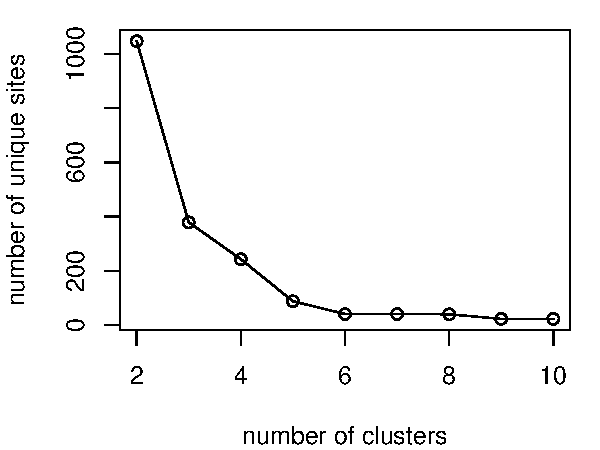
\includegraphics[scale=0.6]{fig_uurls.pdf}\hfill
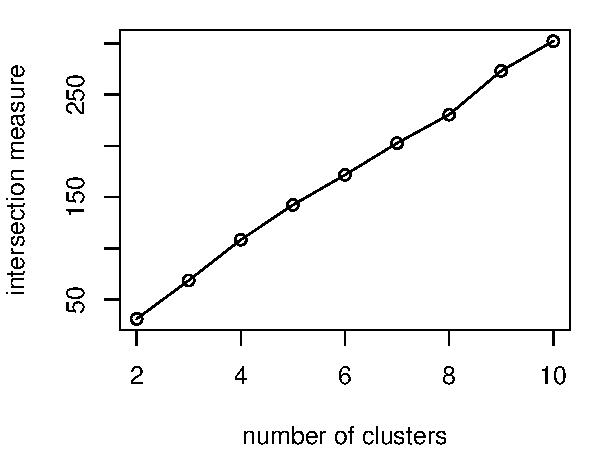
\includegraphics[scale=0.6]{fig_meas.pdf}

\caption{The number-of-unique-sites vs $k$ plot (on the left) and $M_I$ vs $k$ plot (on the right)}
\label{N7Jti}
\end{figure}

Taking into account the aforementioned parameters and after the AIC algorithm results (see \cite{aic}) we select $k=6$. Then the intersection measure $M_I$ is minimized by weights:
\[
	\boldsymbol{w} = (0.4, 0.4, 1.0, 0.4).
\]
Let us recall that the weight $w_3$ corresponds to the age of the user. Due to that we might suggest that the age has the most the most distinguishing effect on the preferences of the users for the Internet sites.


\subsubsection{The results and their interpretation.}

Some information on the resulting clusters are provided in Tables~\ref{OWoti} and~\ref{01Yti}. The Table~\ref{OWoti} contains the demographic composition of the clusters. The Table~\ref{01Yti} contains 10 subject categories of sites (the mapping of sites to the categories were done according to Yandex database \cite{yandex}) most specific to the relevant clusters.


\begin{table}
	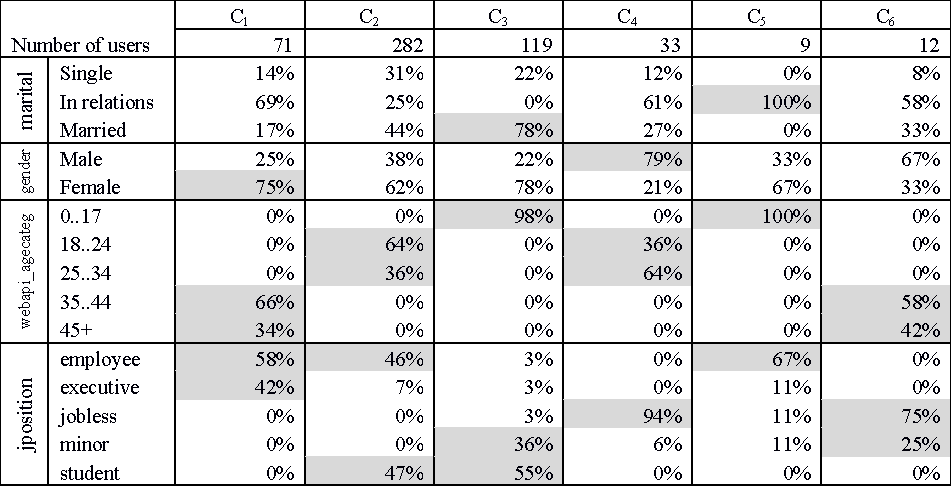
\includegraphics[width=\linewidth]{t1.pdf}
	
	\caption{The demographic composition of the clusters. The most distinctive attribute values for the clusters are greyed out.}
	\label{OWoti}
\end{table}





\begin{table}
	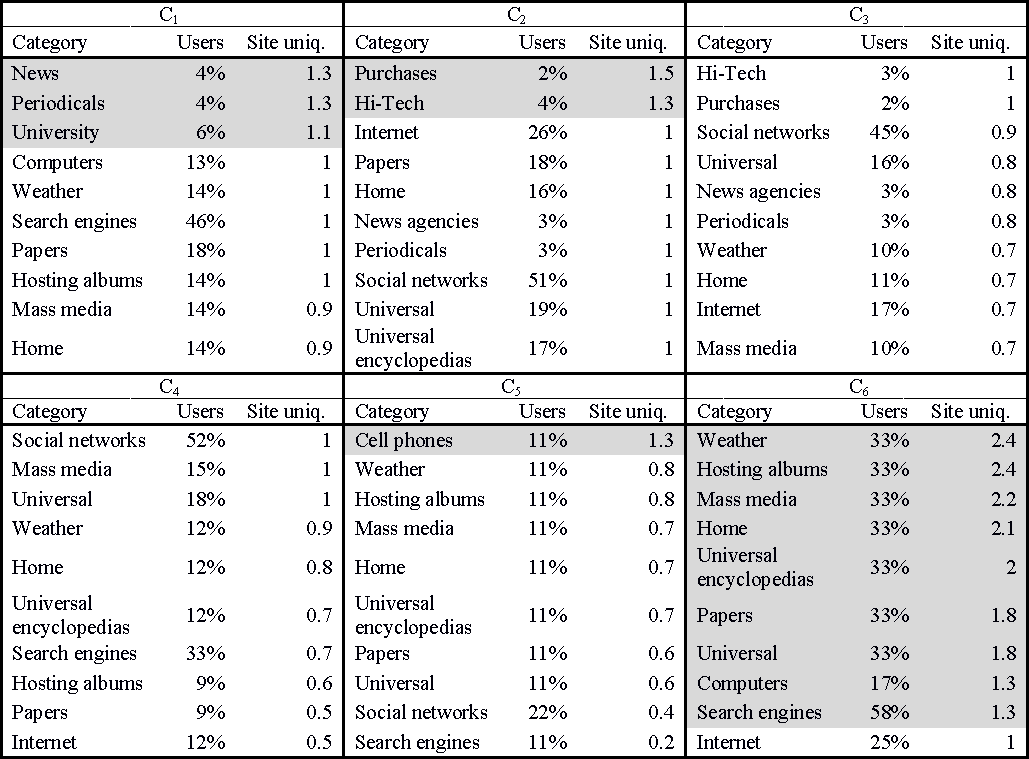
\includegraphics[width=\linewidth]{t2.pdf}
	
	\caption{Some information on web activity of users from each of the cluster. The column ``Users'' shows the proportion of users of the cluster which have visited the sites of the category. The column ``Site uniq.'' shows how many times more in average the sites of the category were visited by users   of the cluster compared to the others.}
	\label{01Yti}
\end{table}

Let us provide a brief description of some of the obtained clusters:
\begin{itemize}
	\item $C_1$ is mostly formed with aged working and unmarried women. It is distinctive for the class to visit news and periodicals sites, and be interested in universities.
    
    \item $C_2$ consists of young/middle-aged students and working people. Their distinctive sites are about Hi-tech and purchases.

	\item $C_5$ consists of working teenagers in relations with high interest in sites about mobile phones.
    
	\item $C_6$ is formed by aged unemployed people with a lot of spare time, as it seems. They are interested in wide variety of website categories, including weather, photo hosts, mass media, home and so on.
\end{itemize}

Let us note that the demographic data on the users were gathered by means of online interview without any validation. For instance, $C_3$ almost completely consists of married people who are under 17 years old which is unlikely to be true. Since these cases cannot be treated as just outliers due to high number, we don't address this issue here.


\section{Analysis for dependencies between the demographic attributes and the websites preferences}



Another goal of our research was testing for the dependencies between the demographic attributes and the website category preferences (the mapping of sites urls to the categories were done according to Yandex database \cite{yandex}). The chi-squared independence test was used since the tested characteristics are qualitative. For every pair of the demographic attribute and website category the contingency tables were built and the independence test was performed with the significance level of $0.05$. To provide better statistical significance, only the categories with more than 1000 visits from distinct users were considered.

Let us note that the categories ``Social networks'' and ``Search engines'' have by far more visits by distinct users than any other category. So the dependencies for these categories could not be detected. This result is evident, as the most popular sites should be visited by all users irrespective of their age, sex and other features. 

Another result is that the likelihood of that an user visits a category doesn't depend on the gender. Perhaps this finding is due to the insufficient sample size.

Some identified dependencies:

\begin{itemize}
	\item Between the \textbf{age} attribute and the category ``\textbf{Newspapers}'' (with a high significance level \textbf{0.0015}). People aged from 0 to 24 years and older than 45 years are much more likely to not visit websites of category ``Newspapers''.

	\item Between the \textbf{marital status} and the category ``\textbf{Dating}'' (the significance level of \textbf{0.026}). The unmarried single persons visit dating websites more often.
	
	\item Between the \textbf{age} attribute and the category ``\textbf{Dating}'' (with a high level of significance \textbf{0.009}). Older people visit dating sites more often than younger.
	
	\item Between the \textbf{age} attribute and the category ``Internet'' (with a high level of significance \textbf{0.01}). It confirms the assumption that young people are more likely to visit websites related to IT.
	
	\item Between the \textbf{age} attribute and the category ``\textbf{Information Agency}'' (with a significance level of \textbf{0.022}). Here it can be seen an unclear relation: young people under 17 years of age significantly more often visit sites of the category News agencies.
	
	\item Between the \textbf{marital status} and the category ``\textbf{Shopping}'' (a high level of importance of \textbf{0.0053}). Single people rarely visit this kind of websites.
	
	\item Between the \textbf{age} attribute and the category ``\textbf{Job}'' (the significance level of \textbf{0.013}). Young people are significantly more interested in the job-search websites.
	
	\item Between the \textbf{age} attribute and the category ``\textbf{Universal Encyclopedia}'' (high significance level \textbf{0.0023}). 
	Young people between 18 and 24 years old visit sites of the category ``Universal Encyclopedia'' more frequently than people of other ages.
	
	\item Between the \textbf{workplace} and the category ``\textbf{Universal Encyclopedia}'' (high significance level \textbf{0.0082}). For this demographic attribute the natural relation is recognized. Students use the sites of this category more often than the other groups. Full-time engineers also use sites of this category more frequently.
	\item Between the \textbf{age} attribute and the category ``\textbf{Humor}'' (significance level \textbf{0.04}). The natural connection is observed. Young people aged from 18 to 34 years visit sites of this category more often.
	\item Between the \textbf{labor} attribute and category ``\textbf{Humor}'' (significance level \textbf{0.03}). Students like the websites of this category.
\end{itemize}


\section{Conclusion}


We have done statistical analysis on some demographic and web activity data. The first part of the statistical investigation was performed using clusterization of weighted demographic data with some special way of weights selecting. The second part consisted in pair-wise testing for the independence between demographic attributes and website preferences of the users. The considered methods allowed to reveal some interesting statistical connections and features of the dataset. It is important to note, that both methods showed somewhat mutually supportive results, namely, they both discovered high influence of age to the websites preferences. This might indicate on the effectiveness of the considered methods.


\subsubsection*{Acknowledgments.} This work was funded by the subsidy allocated to Kazan Federal University for the state assignment in the sphere of scientific activities. 

\begin{thebibliography}{4}


\bibitem{sim-1} 
Sloan, L., Morgan, J., Burnap, P., Williams, M.: Who Tweets? Deriving the Demographic Characteristics of Age, Occupation and Social Class from Twitter User Meta-Data. In: Preis T, ed. PLoS ONE., 10(3) (2015)

\bibitem{sim-2}
Stattner, E., Collard, M.: Clustering of links and clustering of nodes: Fusion of knowledge in social networks. In: Studies in Computational Intelligence, 665, pp. 255-276 (2017)

\bibitem{sim-3}
Zhang, Y., Xu, G., Zhou, X.: A Latent Usage Approach for Clustering Web Transaction and Building User Profile. In: Advanced Data Mining and Applications: First International Conference, ADMA 2005, Wuhan, China, July 22-24, 2005. Proceedings, pp 31--42 (2005)

\bibitem{sim-4}
Zhao, H., He, C.: Objective Cluster Analysis in Value-Based Customer Segmentation Method. In: 2009 Second International Workshop on Knowledge Discovery and Data Mining, Moscow, 2009, pp. 484--487 (2009)

\bibitem{sim-5}
Zhao P., Zhang C.-Q. : A new clustering method and its application in social networks. In: Pattern Recognition Letters, 32, pp. 2109--2118 (2011)

\bibitem{r-project} R Core Team. R: A language and environment for statistical computing. R Foundation for Statistical Computing, Vienna, Austria, https://www.R-project.org/.

\bibitem{hclust} Rokach, Lior, Oded, Maimon: Clustering methods. Data mining and knowledge discovery handbook. Springer US (2005)

\bibitem{aic} Akaike, H.: Information theory and an extension of the maximum likelihood principle. In: 2nd International Symposium on Information Theory, Tsahkadsor, Armenia, USSR, September 2-8, 1971, Budapest: Akadémiai Kiadó, pp. 267–-281 (1973)

\bibitem{yandex} Yandex catalog, https://yandex.com/yaca/



\end{thebibliography}




\end{document}
